\documentclass[12pt]{beamer}
\usepackage[utf8]{inputenc}
\usepackage[T1]{fontenc}
\usepackage{graphicx}
\usepackage{lmodern}
\usetheme{PaloAlto}
\begin{document}
	\author{Leonardo Testolin - VR436823}
	\title{Diverse soluzioni e sfide per gli schermi
		AMOLED e OLED}
	%\subtitle{}
	%\logo{}
	%\institute{}
	%\date{}
	%\subject{}
	%\setbeamercovered{transparent}
	%\setbeamertemplate{navigation symbols}{}
	\begin{frame}[plain]
		\maketitle
	\end{frame}
	
	\begin{frame}
		\frametitle{Introduzione: alcuni concetti base}
		\begin{figure}[h]
			\centering
			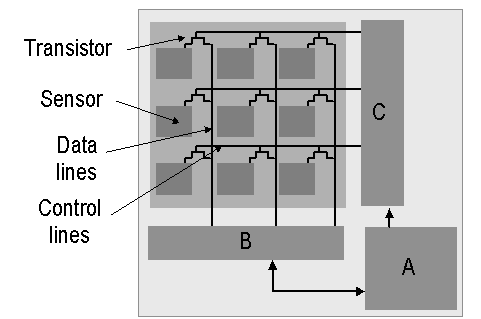
\includegraphics[width=1\textwidth]{IMMAGINI/arraydiag}
			\caption{TFT}
			\label{TFT}
		\end{figure}
	\end{frame}
	\begin{frame}
		\frametitle{Introduzione: alcuni concetti base}
		\begin{figure}
			\centering
			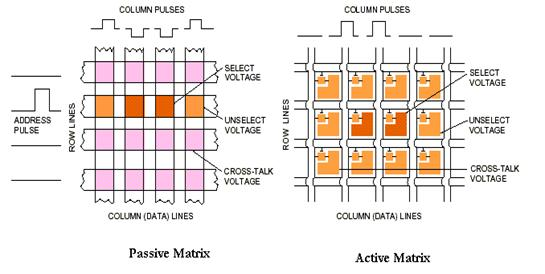
\includegraphics[width=1\linewidth]{IMMAGINI/matrix_passive}
			\caption{ Passive Matrix and Active Matrix}
			\label{fig:matrixpassive}
		\end{figure}
	\end{frame}
	\begin{frame}
		\frametitle{Introduzione: alcuni concetti base}
		\begin{figure}
			\centering
			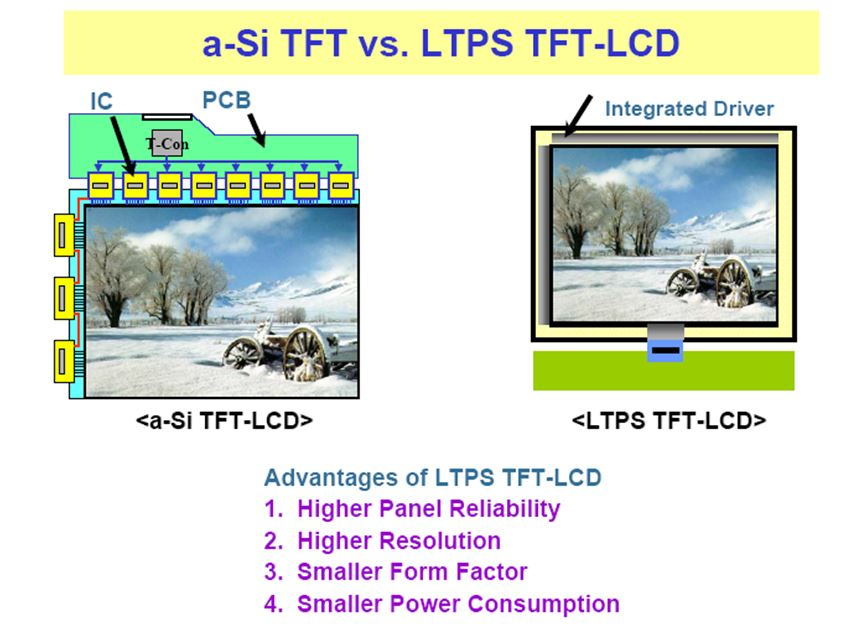
\includegraphics[width=1\linewidth]{IMMAGINI/ltps-(technology)}
			\caption{LTPS-technology}
			\label{fig:ltps-technology}
		\end{figure}
	\end{frame}
	\begin{frame}
		\frametitle{Introduzione: alcuni concetti base}
		\begin{figure}
			\centering
			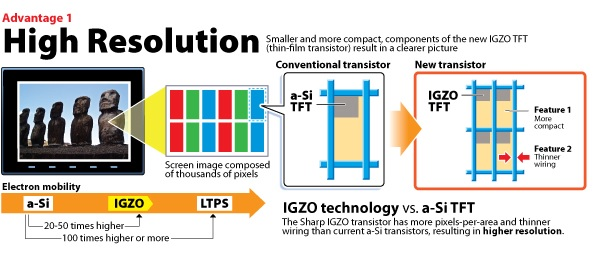
\includegraphics[width=1\linewidth]{IMMAGINI/IGZO-vs-aSi-1}
			\caption{IGZO vs a-Si}
			\label{fig:igzo-vs-asi-1}
		\end{figure}
	\end{frame}
	\begin{frame}
		\frametitle{Introduzione: alcuni concetti base}
		\begin{figure}
			\centering
			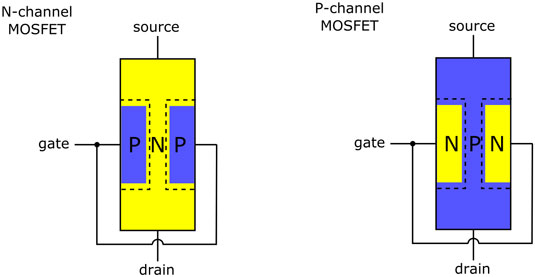
\includegraphics[width=1\linewidth]{IMMAGINI/FET_DET}
			\caption{Transistor FET}
			\label{fig:fetdet}
		\end{figure}
	\end{frame}
	\begin{frame}
		\frametitle{24-INCH WIDE UXGA TFT-LCD per applicazioni HDTV}
		\begin{itemize}
			\item Sorgono molti problemi nella creazione di schermi di grandi dimensioni
			\pause
			\item Molti approcci sono stati adottati per cercare di superare l’insufficienza della ricarica del pannello,
			cercando di usare tecniche guidate, cercando di manipolare il tempo di ricarica
			\pause
			\item Quando pixel e dimensione dello schermo aumentano, il consumo energetico che deve essere fornito ai pixel diventa un problema molto critico
		\end{itemize}
	\end{frame}
	\begin{frame}
		\frametitle{24-INCH WIDE UXGA TFT-LCD per applicazioni HDTV}
		\begin{itemize}
			\item I problemi maggiori sono legati anche a problemi di ritardo e la distorsione data dall'alta resistenza e capacità parassitaria
		\end{itemize}
	\end{frame}
	\begin{frame}
		\frametitle{24-INCH WIDE UXGA TFT-LCD per applicazioni HDTV}
		\begin{figure}
			\centering
			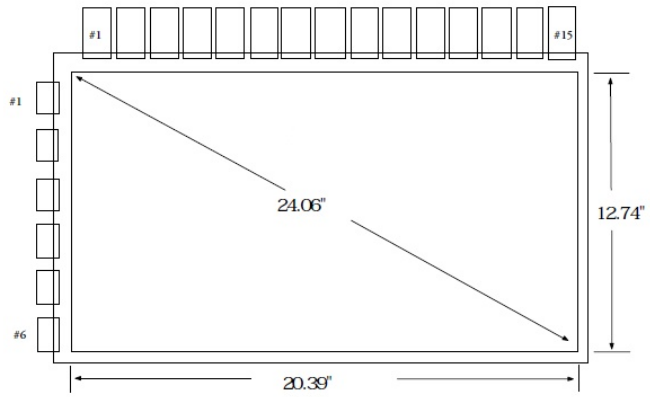
\includegraphics[width=1\linewidth]{IMMAGINI/schermoLCD}
			\caption{Schermo LCD}
			\label{fig:schermolcd}
		\end{figure}
	\end{frame}
	\begin{frame}
		\frametitle{24-INCH WIDE UXGA TFT-LCD per applicazioni HDTV}
		\begin{itemize}
			\item Dall’analisi di alcuni risultati, si è potuto notare che i ritardi sulle gate line  causano insufficienza di carica nei pixel causando lo sfarfallio dello schermo, mentre i ritardi sulle data line causano insufficienza di carica nei pixel relativi al cross-talk verticale
		\end{itemize}
	\end{frame}
	\begin{frame}
	\frametitle{24-INCH WIDE UXGA TFT-LCD per applicazioni HDTV:  Metodi}
		\begin{itemize}
			\item Se ci sono questi problemi è possibile implementare lo split delle data line
			\pause
			\item Si riduce così il clock e il data rate abbastanza
			da usare un device con frequenze molto più basse
			\pause
			\item 4 differenti bus dati sono richiesti per poter gestire questi 4 blocchi dati differenti
		\end{itemize}
	\end{frame}
	\begin{frame}
		\frametitle{24-INCH WIDE UXGA TFT-LCD per applicazioni HDTV:  Metodi}
		\begin{figure}
			\centering
			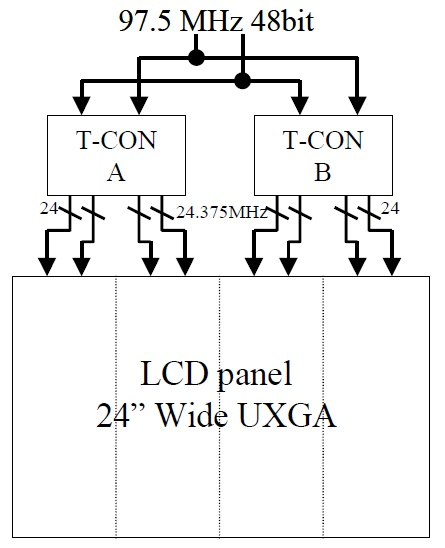
\includegraphics[width=0.5\linewidth]{FISICA/T-CON}
			\caption{T-CON}
			\label{fig:t-con}
		\end{figure}
	\end{frame}
	\begin{frame}
		\frametitle{24-INCH WIDE UXGA TFT-LCD: Configurazione di sistema}
		Un sistema totale usato per un display WUXGA consiste di 3 parti:
		\begin{itemize}
			\item Scheda video
			\item Interfaccia IC
			\item Modulo TFT-LCD di 24-inch
		\end{itemize}
	\end{frame}
	\begin{frame}
		\frametitle{24-INCH WIDE UXGA TFT-LCD: Configurazione di sistema}
		\begin{figure}
			\centering
			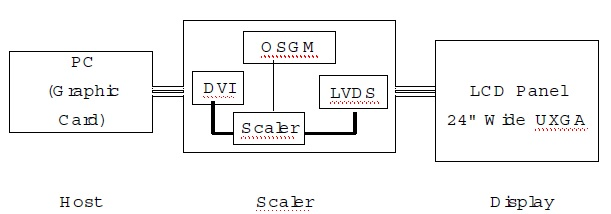
\includegraphics[width=1\linewidth]{FISICA/sistema_di_conf}
			\caption{Configurazione di sistema}
			\label{fig:sistemadiconf}
		\end{figure}
	\end{frame}
	\begin{frame}
		\frametitle{24-INCH WIDE UXGA TFT-LCD: angolo di visione}
		\begin{itemize}
			\item Per migliorare la visione d’angolo dello schermo è stato sviluppato un nuovo
			modello VA (vertical alignment) ridenominato PVA (patterned
			vertical alignment), che utilizza dei campi della frontiera che sono guidati rispettivamente con il modello VA
			\pause
			\item Cosi facendo dopo alcuni test si sono potuti ottimizzare le prestazioni delle celle del display 
		\end{itemize}
	\end{frame}
	\begin{frame}
		\frametitle{Pixel AMOLED basati su circuiti in poly-Si TFTs: introduzione}
		\begin{itemize}
			\item In particolare si fa una comparazione tra accuratezza, velocità di guida, consumo
			energetico e area occupata
		\end{itemize}
	\end{frame}
	\begin{frame}
		\frametitle{Pixel AMOLED basati su circuiti in poly-Si TFTs: introduzione}
		\begin{itemize}
			\item Organic ligth-emitting diode (OLED) sono display che sono efficienti dal punto di vista del consumo energetico,vivido e ideale per applicazioni portatili 
			\pause
			\item Sono costituiti da materiali a basso costo e vengono utlizzati meno processi di produzione per la loro creazione rispetto agli LCDs
		\end{itemize}
	\end{frame}
	\begin{frame}
		\frametitle{Pixel AMOLED basati su circuiti in poly-Si TFTs: introduzione}
		\begin{figure}
			\centering
			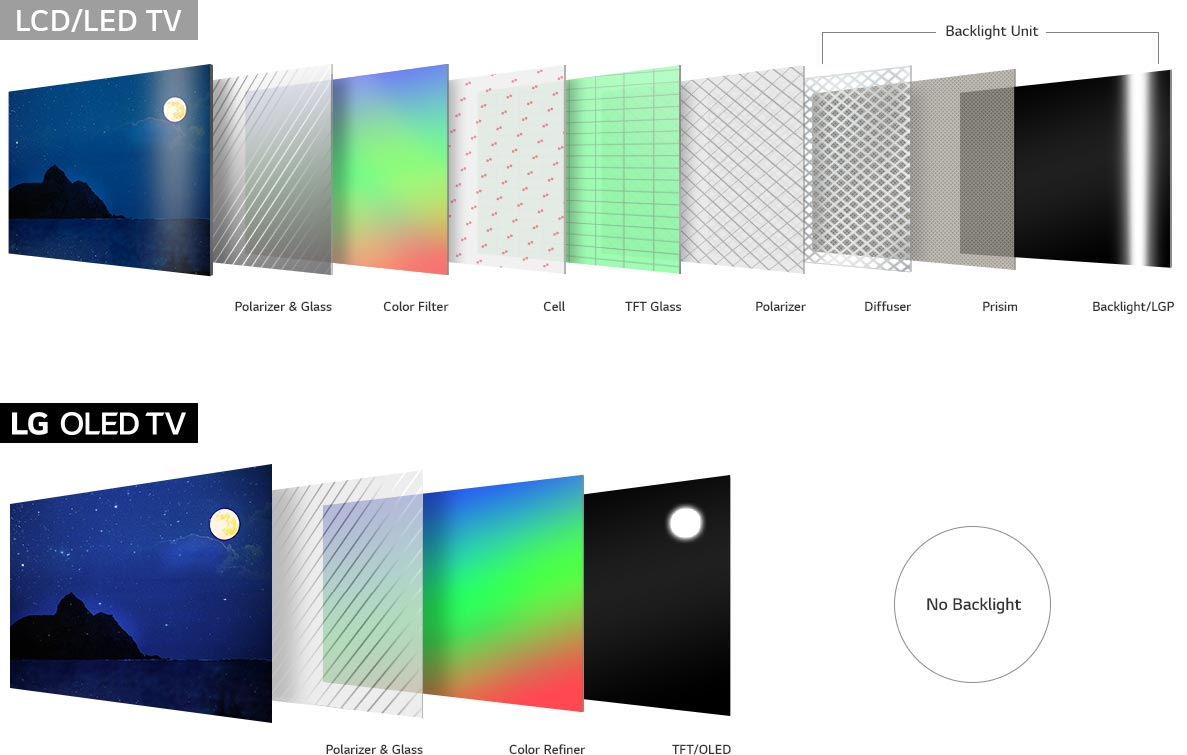
\includegraphics[width=1\linewidth]{IMMAGINI/oled}
			\caption{OLED}
			\label{fig:oled}
		\end{figure}
	\end{frame}
	\begin{frame}
		\frametitle{Pixel AMOLED basati su circuiti in poly-Si TFTs: introduzione}
		\begin{itemize}
			\item L’OLED è un device guidato da corrente dove il livello di luminosità è determinato dal livello di corrente che lo attraversa
		\end{itemize}
	\end{frame}
	\begin{frame}
		\frametitle{Pixel AMOLED basati su circuiti in poly-Si TFTs: introduzione}
		\begin{itemize}
			\item Per queste ragioni gli OLED appaiono i migliori candidati per le diverse applicazioni mobili
			\pause
			\item Questa corrente può essere fornita da una matrice passiva OLED (PMOLED) oppure da una matrice attiva (AMOLED)
		\end{itemize}
	\end{frame}
	\begin{frame}
		\frametitle{Pixel AMOLED basati su circuiti in poly-Si TFTs: introduzione}
		\begin{itemize}
			\item La soluzione proposta prevede un approccio in cui si tende ad utilizzare la matrice passiva, in particolare, quando la dimensione dello schermo va aumentando
			\pause
			\item La matrice passiva richiede un picco elevato di corrente per poter funzionare, ma questo, permette di ottenere alta luminosità
			\pause
			\item Un consumo elevato di energia ha dimostrato effetti di maggior affidabilità da parte degli schermi OLED
		\end{itemize}
	\end{frame}
	\begin{frame}
		\frametitle{Pixel AMOLED basati su circuiti in poly-Si TFTs: Circuiti driver per gli schermi OLED}
		I circuiti OLED possono essere divisi in due classi:
		\begin{itemize}
			\item Circuiti sul voltaggio
			\pause
			\item Circuiti sulla corrente
		\end{itemize}
	\end{frame}
	\begin{frame}
		\frametitle{Pixel AMOLED basati su circuiti in poly-Si TFTs: Voltage-programming driver circuits}
		\begin{itemize}
			\item Il più semplice circuito chiamato 2-TFT, può essere creato tramite due TFT (T1 e T2)
			\pause
			\begin{figure}
				\centering
				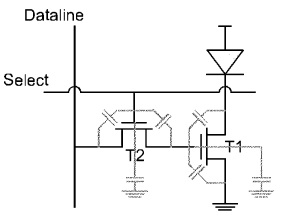
\includegraphics[width=0.7\linewidth]{FISICA/tft_oled_driver}
				\caption{TFT OLED driver}
				\label{fig:tftoleddriver}
			\end{figure}
		\end{itemize}
	\end{frame}
	\begin{frame}
		\frametitle{Pixel AMOLED basati su circuiti in poly-Si TFTs: Voltage-programming driver circuits}
		\textcolor{red}{Problemi:}
		\begin{itemize}
			\item Pesante drenaggio di corrente dovuto alla threshold del TFT
			\item Variazione di mobilità delle cariche
		\end{itemize}
		\pause
		\textcolor{green}{Soluzione:}
		\pause
		\begin{itemize}
			\item Per poter superare questo inconveniente deve essere introdotto un circuito che si auto-compensa, è semplice da realizzare, ma ha bisogno di più componenti
		\end{itemize}
	\end{frame}
	\begin{frame}
		\frametitle{Pixel AMOLED basati su circuiti in poly-Si TFTs: Voltage-programming driver circuits}
		\begin{itemize}
			\item Introducendo questa miglioria, il circuito risultante sarà denominato 4-TFT
		\end{itemize}
		\pause
		\begin{figure}
			\centering
			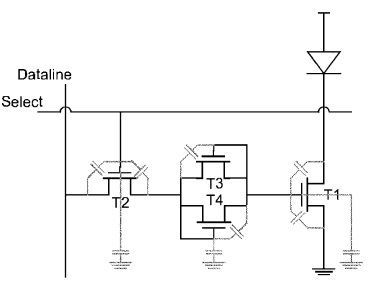
\includegraphics[width=0.7\linewidth]{FISICA/tft_oled_maggiore}
			\caption{TFT OLED major}
			\label{fig:tftoledmaggiore}
		\end{figure}
	\end{frame}
	\begin{frame}
		\frametitle{Pixel AMOLED basati su circuiti in poly-Si TFTs: Current-programming driver circuits}
		Possiamo settare in maniera precisa la corrente che viene data allo schermo OLED con un approccio basato sulla programmazione di corrente
	\end{frame}
	\begin{frame}
		\frametitle{Pixel AMOLED basati su circuiti in poly-Si TFTs: Current-programming driver circuits}
		\begin{figure}
			\centering
			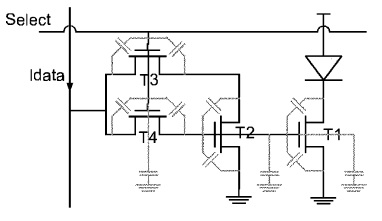
\includegraphics[width=1\linewidth]{FISICA/current_mirror}
			\caption{Current Mirror}
			\label{fig:currentmirror}
		\end{figure}
	\end{frame}
	\begin{frame}
		\frametitle{Pixel AMOLED basati su circuiti in poly-Si TFTs: Current-programming driver circuits}
		Una variante migliore rispetto alla precedente, introduce una circuito driver con memoria. Questo permetterà di ottenere migliori prestazioni in quanto è possibile tenere "in memoria" un certo voltaggio
	\end{frame}
	\begin{frame}
		\frametitle{Pixel AMOLED basati su circuiti in poly-Si TFTs: Current-programming driver circuits}
		\begin{figure}
			\centering
			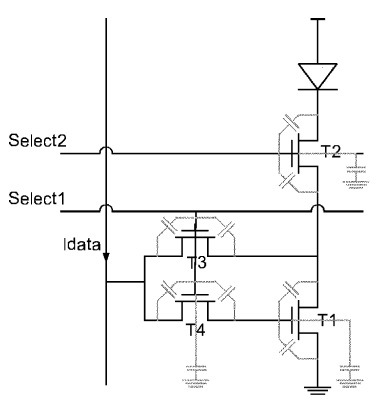
\includegraphics[width=0.6\linewidth]{FISICA/one_tras_current}
			\caption{One-transistor current memory driver circuit}
			\label{fig:onetrascurrent}
		\end{figure}
	\end{frame}
	\begin{frame}
		\frametitle{Pixel AMOLED basati su circuiti in poly-Si TFTs: Velcocità di guida}
		\begin{itemize}
			\item Per calcolare il frame rate dei pixel	si utilizza una formula che considera il numero di righe per matrice, il tempo di ricarica dei capacitori, il tempo di ricarica del capacitore TFT e il tempo di carica e scarica delle righe della matrice
		\end{itemize}
	\end{frame}
	\begin{frame}
		\frametitle{Pixel AMOLED basati su circuiti in poly-Si TFTs: Conclusioni}
		\begin{itemize}
			\item Tra le differenti topologie, la migliore è la 4-TFT con la quale la velocità è 10 volte più alta rispetto alla
			topologia basate su corrente e con un risparmio del 30\% più alto. Però, se il 10\%
			della variazione sul drenaggio della corrente è dovuto alla variazione di mobilità,
			questo non può essere accettato e quindi si passa ad una topologia basata su
			corrente
		\end{itemize}
	\end{frame}
	\begin{frame}
		\frametitle{Display AMOLED pieghevoli: introduzione}
		\begin{itemize}
			\item La fisicità del display risulta essere molto importante in termini di portabilità e design
		\end{itemize}
	\end{frame}
	\begin{frame}
		\frametitle{Display AMOLED pieghevoli: introduzione}
		\begin{itemize}
			\item Ci sono alcuni punti chiave da dover tenere in considerazione quando si parla di display OLED pieghevoli ed è la rottura del display dovuta alla curvatura
			\pause
			\item Di solito,un display OLED include un sottostrato di plastica piuttosto che un sottostrato di vetro
			\pause
			\item La plastica trasmette condensa/umidità; quindi, dei film passivi sono richiesti per poter reagire con l’umidità e la degradazione
		\end{itemize}
	\end{frame}
	\begin{frame}
		\frametitle{Display AMOLED pieghevoli: introduzione}
		\begin{itemize}
			
		\end{itemize}
	\end{frame}
trasmissione del vapore acqueo (WVRT)

	
	
	
	
	
	
	
	
	
	
	
	
	
	
	
	
	
\end{document}